\documentclass[aspectratio=169,10pt]{beamer}
\usetheme{Madrid}
\usecolortheme{default}
\usepackage[T1]{fontenc}
\usepackage{lmodern,amsmath,amssymb,mathtools,booktabs,tikz,etoolbox}
% Add a little breathing room between list entries while keeping slides compact.
\AtBeginEnvironment{itemize}{\setlength{\itemsep}{3pt}\setlength{\parskip}{0pt}}
\AtBeginEnvironment{enumerate}{\setlength{\itemsep}{3pt}\setlength{\parskip}{0pt}}
\AtBeginEnvironment{description}{\setlength{\itemsep}{3pt}\setlength{\parskip}{0pt}}
\usetikzlibrary{arrows.meta,positioning,shapes.geometric,fit,calc}
\setbeamertemplate{navigation symbols}{}
\setbeamertemplate{footline}[frame number]
\title[GridPath Benders]{GridPath and NextGrid Benders Decomposition}
\author{Carl Swanson}
\date{\today}
\tikzset{process/.style={draw,rounded corners,align=center,minimum height=8mm,text width=30mm,fill=blue!7},file/.style={draw,rounded corners,align=center,minimum height=7mm,text width=33mm,fill=green!8,font=\small},decision/.style={draw,diamond,aspect=2,align=center,fill=orange!12,text width=22mm,inner sep=1pt},arrow/.style={-{Stealth[length=2mm]},thick}}
\begin{document}
\begin{frame}\titlepage\end{frame}

\begin{frame}{Purpose and High-level overview}
\textbf{Purpose}
\begin{itemize}
\item The purpose of Benders decomposition is to efficiently solve large-scale planning problems 
by separating investment and policy-allocation decisions from operational evaluations. This allows the 
concurrent solve of temporal and/or stochastic subproblems instead of solving the monolithic model.
\item The primary use case will be to enable hydro modelling. Other benefits include modelling integer 
investment and operational decisions.
\end{itemize}
\textbf{High-level overview}
\begin{itemize}
\item The planning model chooses investment and policy-allocation decisions.
\item Operational subproblems evaluate operating value conditional on those decisions.
\item Workers return recourse values, dual sensitivities, or feasibility information.
\item The master accumulates cuts and chooses the next planning point.
\end{itemize}
\[
\max_{x\in X}\left\{\mathrm{NPV}_{\mathrm{plan}}(x)-\sum_{w\in W}Q_w(x_L)\right\},
\quad Q_w(x_L)=-\max_{z_w\in Z_w(x_L)}\mathrm{OP\_NPV}_w(z_w).
\]
\end{frame}
\section{Quick start and essential information}

\begin{frame}{Quick start and essential information}
\small
\begin{block}{Minimum Benders command}
\texttt{gridpath\_run --scenario YOUR\_SCENARIO --benders 1}
\end{block}
\begin{itemize}
\item Run from the intended Python environment after installing this GridPath checkout and preparing the scenario inputs.
\item \texttt{--scenario} names the scenario directory. By default it is found under \texttt{../scenarios}; use \texttt{--scenario\_location} to set a different parent directory.
\item \texttt{--benders 1} selects Benders decomposition. The flag is required; \texttt{0} selects the ordinary solve path.
\item Select the solver with \texttt{--solver}; ensure its executable and licence are available. The scenario's \texttt{solver\_options.csv} may also configure the solver.
\item \texttt{--n\_parallel\_solve} controls concurrent operational workers. Increase it only with sufficient memory, CPU capacity, and solver licences.
\item Check the installed command and option spellings with \texttt{gridpath\_run --help}.
\end{itemize}
\end{frame}

\begin{frame}{Essential Benders CLI options: algorithm controls}
\scriptsize
\begin{tabular}{@{}p{0.43\textwidth}p{0.49\textwidth}@{}}
\toprule Option (default) & What it controls \\
\midrule
\texttt{--max\_benders\_iter} (200) & Maximum number of master--worker iterations. \\
\texttt{--benders\_conv\_tol} ($10^{-10}$) & Relative UB--LB convergence tolerance. \\
\texttt{--benders\_abs\_gap\_tol} ($10^{-4}$) & Absolute UB--LB gap tolerance, in objective units. \\
\texttt{--max\_benders\_cpu\_time} (3600) & CPU-time limit passed to each operational subproblem solve configuration, in seconds. \\
\texttt{--benders\_master\_discrete\_method} (\texttt{pj\_relax}) & Master integer handling: \texttt{pj\_relax}, \texttt{linearized}, \texttt{djc}, or \texttt{none}. DJC requires native MOSEK. \\
\texttt{--benders\_operational\_discrete\_method} (\texttt{fixed\_z}) & Treatment of non-linking operational integers: fix the integer state for dual cuts (\texttt{fixed\_z}) or relax integrality (\texttt{pj\_relax}). \\
\texttt{--benders\_use\_pj\_initialization} (true) & Use Pecci--Jenkins initialization when there are no discrete linking variables. \\
\bottomrule
\end{tabular}
\end{frame}

\begin{frame}{Essential Benders CLI options: stabilization and execution}
\scriptsize
\begin{tabular}{@{}p{0.43\textwidth}p{0.49\textwidth}@{}}
\toprule Option (default) & What it controls \\
\midrule
\texttt{--benders\_stabilization\_method} (\texttt{none}) & Trial-point selection: no L1/L2 distance objective, weighted L1 distance, or weighted L2 distance. With the default nonzero level parameter, \texttt{none} still uses Pecci--Jenkins level-set regularization. \\
\texttt{--benders\_stab\_param} (0.025) & Level-set parameter $\gamma$; controls how tightly the trial point is restricted relative to the current UB--LB gap. L1/L2 require a nonzero value. \\
\texttt{--benders\_stab\_dynamic} (true) & Adapt $\gamma$ during iterations; set false to keep it fixed. \\
\texttt{--benders\_operational\_solver} (\texttt{automatic}) & LP algorithm for MOSEK/Gurobi operational relaxations: \texttt{automatic}, \texttt{interior\_point}, or \texttt{primal\_simplex}. \\
\texttt{--benders\_skip\_final\_export} (off) & Skip the final worker solves and per-subproblem exports at the best incumbent. Planning and convergence outputs are still written. \\
\texttt{--n\_parallel\_solve} (1) & Number of operational subproblems solved concurrently. \\
\texttt{--solver} (HiGHS if otherwise unspecified) & Pyomo solver interface for the master and selected Benders backend. Match the solver to the requested discrete method and installed integration. \\
\bottomrule
\end{tabular}
\vspace{1mm}
\begin{itemize}
\item Boolean options accept true/false, t/f, yes/no, y/n, and 1/0.
\item The implementation accepts \texttt{none} and \texttt{linearized} for the master discrete method even though the parser help text currently advertises only \texttt{pj\_relax} and \texttt{djc}.
\end{itemize}
\end{frame}

\begin{frame}{Key files}
\scriptsize
\begin{tabular}{@{}p{0.37\textwidth}p{0.56\textwidth}@{}}
\toprule File & Responsibility\\\midrule
\texttt{algorithms.py} & Driver loop, workers, bounds, cuts, discrete states, convergence\\
\texttt{planning.py} & Master objective, theta variables, cut lists, solve and extraction\\
\texttt{operational\_model\_creation.py} & Worker model creation and linking-variable identification\\
\texttt{subproblems.py} & Persistent workers, linking rows, recourse solves, duals\\
\texttt{restoration.py} & Phase-I restoration and dual certificate\\
\texttt{regularization.py} & Level-set problem, L1 and L2 stabilization\\
\texttt{soc\_allocation.py} & Storage SOC allocation variables and targets\\
\texttt{benders\_policy\_constraint.py} & Master policy-allocation and SOC constraints\\
\texttt{mosek\_benders.py} & Native MOSEK DJC support\\
\texttt{run\_scenario.py} & Scenario entry point and result exports\\
\bottomrule
\end{tabular}
\end{frame}

\begin{frame}{Algorithm flowchart: one Benders iteration}
\centering
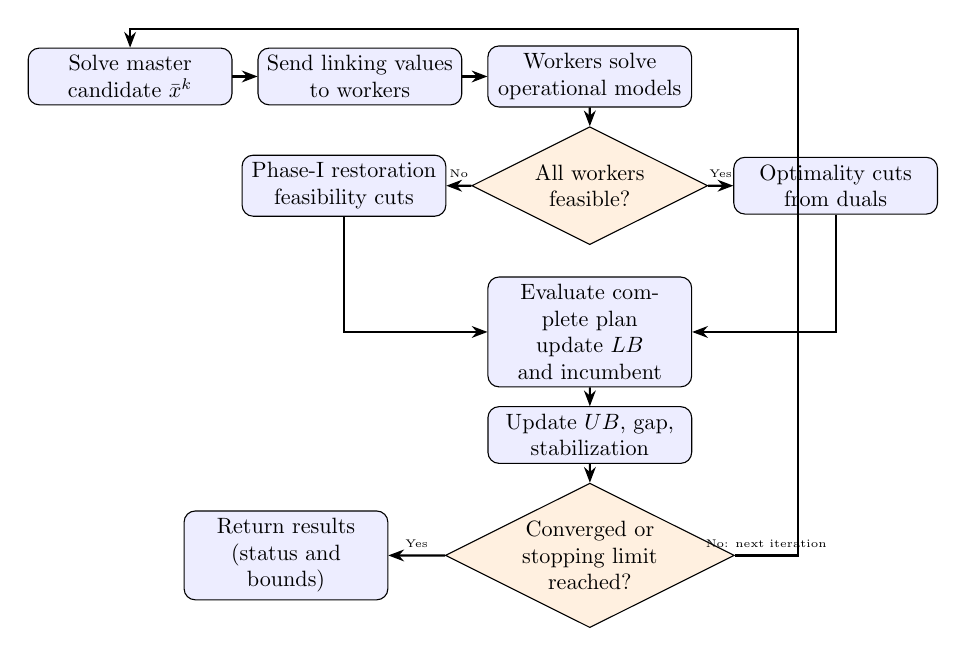
\begin{tikzpicture}[
    node distance=3mm and 4mm,
    scale=.8,
    transform shape
]
\node[process] (master) {Solve master\\candidate $\bar{x}^k$};
\node[process,right=of master] (send) {Send linking values\\to workers};
\node[process,right=of send] (solve) {Workers solve\\operational models};
\node[decision,below=of solve] (feas) {All workers\\feasible?};
\node[process,left=of feas] (rest) {Phase-I restoration\\feasibility cuts};
\node[process,right=of feas] (opt) {Optimality cuts\\from duals};
\node[process,below=of feas,yshift=-2mm] (inc) {Evaluate complete plan\\update $LB$ and incumbent};
\node[process,below=of inc] (bound) {Update $UB$, gap,\\stabilization};
\node[decision,below=of bound] (stop) {Converged or\\stopping limit reached?};
\node[process,left=of stop,xshift=-5mm] (done) {Return results\\(status and bounds)};

\draw[arrow] (master) -- (send);
\draw[arrow] (send) -- (solve);
\draw[arrow] (solve) -- (feas);
\draw[arrow] (feas) -- node[above,font=\tiny]{No} (rest);
\draw[arrow] (feas) -- node[above,font=\tiny]{Yes} (opt);
\draw[arrow] (rest) |- (inc);
\draw[arrow] (opt) |- (inc);
\draw[arrow] (inc) -- (bound);
\draw[arrow] (bound) -- (stop);
\draw[arrow] (stop) -- node[above,font=\tiny]{Yes} (done);

% Return to the master for the next iteration.
\draw[arrow] (stop.east) -- node[above,font=\tiny]{No: next iteration} ++(10mm,0)
    |- ([yshift=3mm]master.north) -- (master.north);

\end{tikzpicture}
\end{frame}

\begin{frame}{Master problem}
\small
\[
\begin{aligned}
\max_{x,\vartheta}\quad&
\mathrm{NPV}_{\mathrm{plan}}(x)-S\sum_{w\in W}\vartheta_w\\
\text{s.t.}\quad&x\in X_{\mathrm{master}},\\
&\vartheta_w\geq L_w/S &&\forall w\in W,\\
&\vartheta_w\geq \frac{Q_w(\bar{x}^{k})}{S}
+\sum_{i\in I_w^k}\frac{\lambda_{w,i}^{k}}{S}(x_i-\bar{x}_i^k)
&&\forall w,\ k\in K_w^{\mathrm{opt}},\\
&c_w^k\bar{s}_w^k+\sum_{i\in I_w^k}\mu_{w,i}^k(x_i-\bar{x}_i^k)\leq0
&&\forall w,\ k\in K_w^{\mathrm{feas}}.
\end{aligned}
\]
\begin{itemize}
\item $\vartheta_w$ is real and has no upper bound.
\item $L_w/S$ and generated cuts provide lower bounds.
\item Original GridPath planning constraints and domains are retained, except for documented relaxations and safeguards.
\end{itemize}
\end{frame}

\begin{frame}{Mathematical objects}
\small
\begin{tabular}{@{}ll@{}}
\toprule Symbol & Meaning\\\midrule
$x$ & All planning/master variables\\
$x_L\subseteq x$ & Linking variables shared with operational workers\\
$\vartheta_w$ & Master approximation of recourse cost for worker $w$\\
$Q_w(x_L)$ & Operating cost, equal to negative operational NPV\\
$W$ & Set of operational subproblem keys\\
$S$ & Scaling constant, $10^9$\\
$L_w$ & Global lower bound on recourse cost for worker $w$\\
$\lambda_{w,i}$ & Optimality-cut sensitivity for linking variable $i$\\
$\bar{s}_w,\mu_{w,i}$ & Phase-I slack and feasibility-cut sensitivities\\
$UB,LB$ & Master upper bound and best evaluated complete-plan lower bound\\
\bottomrule
\end{tabular}
\[
\vartheta_w\approx Q_w(x_L)/S;\quad
\text{master objective}=\mathrm{NPV}_{\mathrm{plan}}-S\sum_w\vartheta_w.
\]
\end{frame}

\begin{frame}{Which variables link master and workers?}
\begin{columns}[T]
\column{0.49\textwidth}\textbf{Capacity and build decisions}
\begin{itemize}\item Generation capacity/build\item Transmission capacity/build\item Storage power and energy capacity\end{itemize}
\column{0.49\textwidth}\textbf{Policy-allocation decisions}
\begin{itemize}\item Emissions and energy targets\item Performance-standard budgets\item Carbon-credit demand/supply/threshold allocations\item Transmission-direction targets\item Fuel-burn and capacity-factor limits\item Yearly storage start/end SOC allocations\end{itemize}
\end{columns}
\end{frame}

\begin{frame}{Software architecture: entry point and driver}
\centering
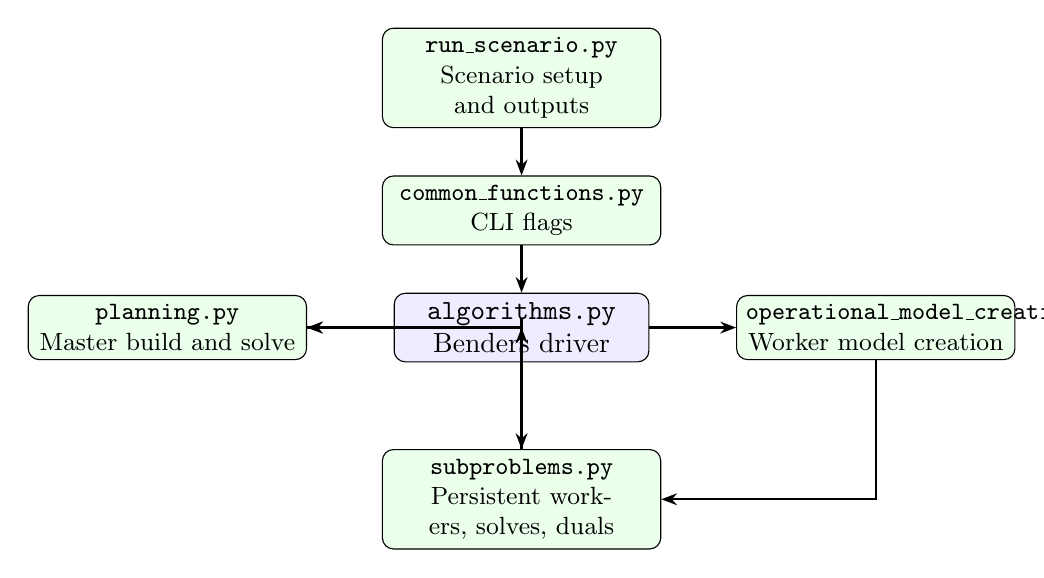
\begin{tikzpicture}[node distance=6mm and 8mm]
\node[file] (run) {\texttt{run\_scenario.py}\\Scenario setup and outputs};
\node[file,below=of run] (common) {\texttt{common\_functions.py}\\CLI flags};
\node[process,below=of common] (driver) {\texttt{algorithms.py}\\Benders driver};
\node[file,left=of driver,xshift=-3mm] (plan) {\texttt{planning.py}\\Master build and solve};
\node[file,right=of driver,xshift=3mm] (create) {\texttt{operational\_model\_creation.py}\\Worker model creation};
\node[file,below=of driver,yshift=-5mm] (sub) {\texttt{subproblems.py}\\Persistent workers, solves, duals};
\draw[arrow](run)--(common);\draw[arrow](common)--(driver);
\draw[arrow](driver)--(plan);\draw[arrow](driver)--(create);
\draw[arrow](create)|-(sub);\draw[arrow](driver)--(sub);
\draw[arrow](sub)|-(plan);\draw[arrow](plan)-|(driver);
\end{tikzpicture}
\end{frame}

\begin{frame}{Software architecture: supporting modules}
\centering
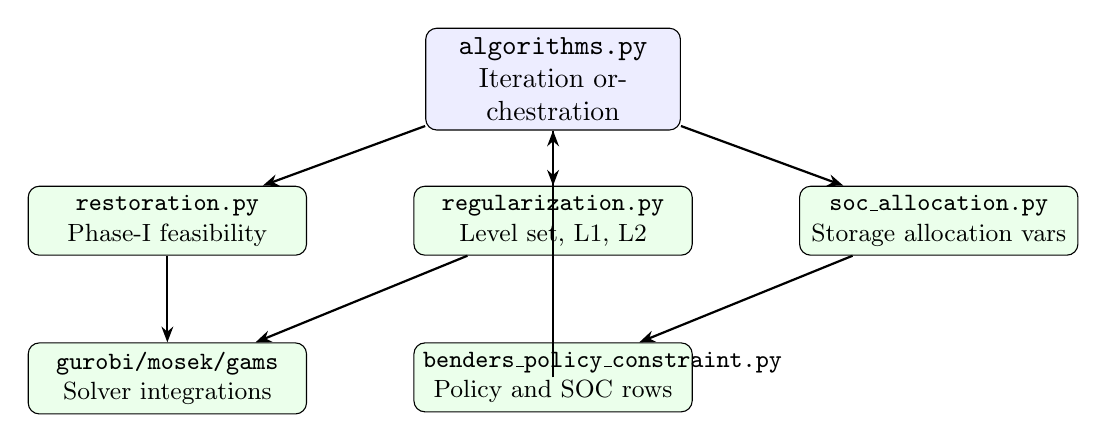
\begin{tikzpicture}[node distance=7mm and 8mm]
\node[process] (driver) {\texttt{algorithms.py}\\Iteration orchestration};
\node[file,below left=of driver,xshift=-7mm] (restore) {\texttt{restoration.py}\\Phase-I feasibility};
\node[file,below=of driver] (reg) {\texttt{regularization.py}\\Level set, L1, L2};
\node[file,below right=of driver,xshift=7mm] (soc) {\texttt{soc\_allocation.py}\\Storage allocation vars};
\node[file,below=of restore,yshift=-4mm] (solver) {\texttt{gurobi/mosek/gams}\\Solver integrations};
\node[file,below=of reg,yshift=-4mm] (policy) {\texttt{benders\_policy\_constraint.py}\\Policy and SOC rows};
\draw[arrow](driver)--(restore);\draw[arrow](driver)--(reg);\draw[arrow](driver)--(soc);
\draw[arrow](restore)--(solver);\draw[arrow](reg)--(solver);
\draw[arrow](soc)--(policy);\draw[arrow](policy)-|(driver);
\end{tikzpicture}
\end{frame}

\begin{frame}{Worker lifecycle and recourse evaluation}
\begin{enumerate}
\item Build one operational model in each persistent worker process.
\item Relax operational integrality and solve a global LP relaxation to obtain operating-NPV upper bound $U_w$.
\item Set $L_w=-U_w$ and report worker readiness.
\item Receive the master's linking-variable point $\bar{x}_L$ each iteration.
\item Add linking equalities $x_i=\bar{x}_i$ as constraints, preserving dual values.
\item Solve the operational LP; for integer operations, solve/fix the integer state and re-solve an LP for duals.
\item Return $Q_w(\bar{x})$, sensitivities, and state information—or invoke Phase-I restoration.
\end{enumerate}
\end{frame}

\begin{frame}{Optimality and feasibility cuts}
\small
\textbf{Optimality cut.} For LP recourse, $Q_w$ is convex and its supporting hyperplane underestimates it:
\[
Q_w(x_L)\geq Q_w(\bar{x}_L^k)+
\sum_{i\in I_w^k}\lambda_{w,i}^k(x_i-\bar{x}_i^k).
\]
The master imposes $\vartheta_w$ above this expression divided by $S$.

\vspace{2mm}
\textbf{Feasibility cut.} A Phase-I problem minimizes a common scaled violation $s_{\max}\geq0$. Its duals provide:
\[
c_w^k\bar{s}_w^k+
\sum_{i\in I_w^k}\mu_{w,i}^k(x_i-\bar{x}_i^k)\leq0.
\]
This excludes trial points certified infeasible by the restoration problem.
\end{frame}

\begin{frame}{Stabilization: level set, L1, and L2}

\[
\ell=UB-\gamma(UB-LB),\qquad
\mathrm{MasterObjective}(x,\vartheta)\geq\ell.
\]

\begin{itemize}
\setlength{\itemsep}{5mm}

\item \textbf{L1:} minimize $\sum_i w_i|x_i-\bar{x}_i|$, represented with positive/negative deviation variables.

\item \textbf{L2:} minimize $\sum_i w_i(x_i-\bar{x}_i)^2$, using a quadratic/conic epigraph path for MOSEK.

\item Only continuous linking variables are penalized; the centre is the last point evaluated by workers.

\item Stabilization chooses the next trial point; it does not replace the master bound or cuts.

\end{itemize}
\end{frame}

\begin{frame}{Bounds: initialization versus safeguard}
\small
\begin{description}
\item[Ordinary initialization] Workers return $U_w$, an upper bound on operating NPV. Set $L_w=-U_w$ and impose $\vartheta_w\geq L_w/S$. The first full master objective initializes $UB$.
\item[Pecci--Jenkins initialization] The temporary planning-only objective is not a bound on the full problem. Therefore $UB=+\infty$ during feasibility restoration; a full master solve initializes a valid $UB$ afterwards.
\item[Running upper bound] After full master solves, update $UB\leftarrow\min(UB,UB_{\mathrm{new}})$.
\item[Emergency variable cap] Only after an unbounded master result, eligible continuous planning variables without an upper bound may be capped at $10^8$. This is an arbitrary safeguard, not the algorithmic $UB$ or a proven physical limit.
\end{description}
\end{frame}

\begin{frame}{Implementation cautions}
\begin{itemize}
\setlength{\itemsep}{8pt}
\item The $10^8$ cap can loosen $U_w$, make $L_w$ more negative, and inflate big-$M$ values.
\item Feasibility restoration relies on an LP dual certificate; unfixed non-linking integer variables are unsupported for that certificate.
\item A newly constructed Pyomo solver interface is a wrapper retry, not proof of a clean external solver process.
\item The code re-solves the updated Pyomo model after adding cuts; internal warm-start or process reuse is solver-interface dependent.
\end{itemize}
\end{frame}

\appendix
\section{Appendix: discrete decisions and conic stabilization}

\begin{frame}{Appendix: master discrete-variable methods}
\small
The master may contain discrete linking variables. A worker cut generated at one discrete state is generally valid only at that state, so the master must enforce the appropriate state condition.

\begin{itemize}
\item \textbf{\texttt{pj\_relax}:} begin with a master in which integer/binary domains are relaxed. After the continuous phase, restore integrality and continue using state-conditioned cuts. This is the Pecci--Jenkins strategy.
\item \textbf{\texttt{linearized}:} use the relaxed phase, then activate each generated cut only when the discrete linking variables match the state at which its worker subproblem was solved. The activation is represented with mismatch indicators and a calculated Big-$M$.
\item \textbf{\texttt{djc}:} use a native MOSEK disjunctive constraint to express the same state-conditioned logic without an explicit Big-$M$ in that disjunction.
\item \textbf{\texttt{none}:} intended for a master with continuous linking variables only. If discrete linking variables are present, the implementation falls back to \texttt{pj\_relax}.
\end{itemize}
\vspace{1mm}
\textbf{Important distinction:} \texttt{--benders\_master\_discrete\_method} controls discrete linking variables in the master. It is separate from \texttt{--benders\_operational\_discrete\_method}, which controls non-linking integer variables inside operational subproblems.
\end{frame}

\begin{frame}{Appendix: state-conditioned cuts with mismatch indicators}
\small
Let $\hat d$ denote the discrete state at which a worker cut was generated, and let $d$ be the master state. For each binary linking variable, define a mismatch indicator:
\[
m_i =
\begin{cases}
1-d_i, & \hat d_i=1,\\
d_i, & \hat d_i=0.
\end{cases}
\]
For general integer linking variables, the implementation uses below/above mismatch indicators relative to the recorded integer value. An aggregate binary indicator $\delta$ is constrained by
\[
\delta\geq m_i\quad\forall i,\qquad
\delta\leq\sum_i m_i.
\]
Thus $\delta=0$ exactly when every discrete variable matches the recorded state; otherwise $\delta=1$.

Write the state-specific Benders inequality as
\[
C(d,x,\vartheta)\geq0.
\]
The linearized activation is
\[
C(d,x,\vartheta)+M\delta\geq0.
\]
When the state matches, $\delta=0$ and the original cut is enforced. When it differs, $\delta=1$ and the calculated $M$ relaxes the cut. The implementation calculates $M$ using the recourse lower bound and bounds on the continuous linking variables; it does not use an arbitrary user-selected constant.
\end{frame}

\begin{frame}{Appendix: native DJCs and operational integer treatment}
\small
\textbf{Native MOSEK disjunctive constraints (DJC)}
\[
\left[
\begin{array}{c}
d=\hat d\\
C(d,x,\vartheta)\geq0
\end{array}
\right]
\quad\lor\quad
[d\neq\hat d].
\]
This is the logical meaning of the state-conditioned cut: enforce the cut at its generating state, or allow a different discrete state. The current native implementation supports binary discrete linking states only and requires the direct native MOSEK interface. It does not support general-integer states through this DJC path.

\medskip
\textbf{Operational non-linking integer variables}
\begin{itemize}
\item \texttt{fixed\_z}: fix the operational integer state for the LP solve used to obtain dual sensitivities. The resulting cut is conditional on that fixed state.
\item \texttt{pj\_relax}: relax operational integrality and obtain duals from the resulting LP relaxation.
\end{itemize}
These operational choices are independent of the master discrete method. Phase-I feasibility restoration also requires an LP dual certificate; unfixed non-linking integer variables are not supported in that restoration certificate.
\end{frame}

\begin{frame}{Appendix: L2 stabilization as a rotated-cone program}
\small
For continuous linking variables $x_i$, centre $\bar x_i$, and nonnegative weights $w_i$, the L2 trial-point objective is
\[
\min_x\quad \sum_{i\in I_{\mathrm{stab}}}w_i(x_i-\bar x_i)^2.
\]
Introduce an epigraph variable $t\geq0$. The equivalent epigraph problem is
\[
\min_{x,t}\quad t
\qquad\text{s.t.}\qquad
t\geq\sum_{i\in I_{\mathrm{stab}}}w_i(x_i-\bar x_i)^2.
\]
Define the rotated quadratic cone
\[
\mathcal Q_r^{n+2}
=
\left\{(u,v,z):
u\geq0,\ v\geq0,\ 2uv\geq\|z\|_2^2
\right\}.
\]
Set
\[
u=t,\qquad v=\frac12,\qquad
z_i=\sqrt{w_i}(x_i-\bar x_i).
\]
Then the epigraph constraint is exactly
\[
\boxed{\left(t,\frac12,
\left[\sqrt{w_i}(x_i-\bar x_i)\right]_{i\in I_{\mathrm{stab}}}
\right)\in\mathcal Q_r^{n+2}.}
\]
Indeed, $2t(1/2)\geq\sum_iw_i(x_i-\bar x_i)^2$ is precisely the required inequality. Minimizing $t$ therefore reproduces the weighted L2 objective exactly.
\end{frame}

\begin{frame}{Appendix: implementation of the L2 cone}
\small
The Pyomo model creates a nonnegative epigraph variable $t$ and records the stabilization variables, weights, and centre values. The custom MOSEK interface then creates affine expressions
\[
y_0=t,\qquad y_1=\frac12,\qquad
y_{i+2}=\sqrt{w_i}\,x_i-\sqrt{w_i}\,\bar x_i,
\]
and places the vector $(y_0,y_1,y_2,\ldots,y_{n+1})$ in a rotated quadratic cone.

\begin{itemize}
\item The cone is an exact representation, not a relaxation or approximation.
\item Nonnegative weights are required; zero weights simply contribute zero.
\item The centre $\bar x$ is the last evaluated planning point, and only the continuous linking variables supplied to the stabilization routine are included.
\item The quadratic expression is used directly when the conic path is not selected. The custom MOSEK path uses the rotated-cone epigraph to avoid expanding large reference values into a quadratic objective.
\end{itemize}
\end{frame}

\begin{frame}{Selected references}
\footnotesize
\begin{thebibliography}{9}
\bibitem{Benders1962} Benders, J. F. (1962). Partitioning procedures for solving mixed-variables programming problems. \emph{Numerische Mathematik}, 4, 238--252.
\bibitem{Geoffrion1972} Geoffrion, A. M. (1972). Generalized Benders decomposition. \emph{JOTA}, 10, 237--260.
\bibitem{Jacobson2024} Jacobson, A., Pecci, F., Sepulveda, N., Xu, Q., and Jenkins, J. D. (2024; online 2023). A computationally efficient Benders decomposition for energy systems planning problems with detailed operations and time-coupling constraints. \emph{INFORMS Journal on Optimization}, 6(1), 32--45.
\bibitem{PecciJenkins2025} Pecci, F. and Jenkins, J. D. (2025). Regularized Benders decomposition for high performance capacity expansion models. \emph{IEEE Transactions on Power Systems}, 40(4), 3105--3116.
\bibitem{Codato2006} Codato, G. and Fischetti, M. (2006). Combinatorial Benders' cuts for mixed-integer linear programming. \emph{Operations Research}, 54(4), 756--766.
\bibitem{Hooker2003} Hooker, J. N. and Ottosson, G. (2003). Logic-based Benders decomposition. \emph{Mathematical Programming}, 96, 33--60.
\bibitem{Balas1979} Balas, E. (1979). Disjunctive programming. \emph{Annals of Discrete Mathematics}, 5, 3--51.
\bibitem{Ruszczynski1986} Ruszczyński, A. (1986). A regularized decomposition method for minimizing a sum of polyhedral functions. \emph{Mathematical Programming}, 35, 309--333.
\bibitem{Rahmaniani2017} Rahmaniani, R. et al. (2017). The Benders decomposition algorithm: A literature review. \emph{European Journal of Operational Research}, 259(3), 801--817.
\end{thebibliography}
\end{frame}
\end{document}
